\documentclass[a4paper]{article}

\usepackage[italian]{babel}
\usepackage[utf8]{inputenc}
\usepackage{amsmath}
\usepackage{graphicx}
\usepackage[colorinlistoftodos]{todonotes}
\usepackage{fullpage}

\title{Analisi delle reti sociali applicata al romanzo Il trono di Spade}

\author{Daniele Baschieri}

\date{\today}

\begin{document}
\maketitle

\begin{abstract}
Your abstract.
\end{abstract}

\section{Introduzione}

In questa relazione si è applicato la metodologia della analisi delle reti sociali al volume Il trono di spade di George R. R. Martin. L'intento era di valutare la versatilità di questo approccio alle più disparate condizioni di utilizzo e estrapolare dal testo elementi realtivi al ruolo e agli eventi grazie a questa tecnica.\\
L'analisi delle reti sociali è una moderna metodologia di analisi delle relazioni proposta da Jacob Levi Moreno fondatore della sociometria. 
Con questa modalità di ricerca si supera il precendente apporccio basato su casi ovvero sulle proprietà di ciascun elemento, e si passa ad un approccio connessionista o strutturalista, ovvero basato su collegamenti con altri elmenti.\\
L'approccio strutturalista permette di catturare il ruolo che un certo elemento ricopre all'interno della rete in funzione di come si relaziona agli altri elementi della rete.\\
L'approccio connessionista invece è basato su flussi e relazioni, questi possono virtualmente rappresentare il guadagno relativo a ciascuna connessione permettendo pratiche misure di potere.\\
Vi è una difficoltà intrinseca nell'analizzare un volume di più di mille pagine, in primo luogo la dimensione del volume che rende obbligatoria una analisi automatica, in secondo luogo l'enrome numero dei personaggi più di un centinaio tra i personaggi rilevanti, infine trovare una misura corretta per rappresentare la rete nel modo più obiettivo possibile, senza quindi sprocare il dato con troppe considerazioni personali.

\section{Obiettivi}

Poichè è possibile piegare la rete a mostrare un infinità di informazioni interessanti si è scelto di limitare la ricerca a due domande fondamentali:

\begin{itemize}
\item La divisione in casate riesce a spiegare la rete sociale tra i personaggi?
\item La relazione matrimoniale dei personaggi riesce a spiegarne la rete sociale?
\end{itemize}
Da queste due domande principali si diramano alcune considerazioni, secondarie ma altrettanto importanti:

\begin{itemize}
\item Quali tensionamenti emergono dalle reti sociali così definite?
\item Chi sono i personaggi chiave del romanzo?
\item Analizzando lo sviluppo della vicenda è possibile prevedere i personaggi che verranno uccisi da una congiura? E il loro assassino?
\end{itemize}

\section{Metodologia}

Per poter lavorare su un volume di quasi 1000 pagine è stato necessario definire con estrema cura il metodo di indagine.\\
Si è quindi pensato di definire i personaggi principali del volume tralasciando solo le comparse, prendendo in esame quindi un elenco con i 105 personaggi più importanti tra quelli riportati nelle appendici di fine libro. Per ciascuno di questi personaggi è stato individuato il nome, il titolo e qualsiasi riferimento nel testo che li caratterizzi in modo univoco.\\
\newtheorem{xxx}{Esempio}
Ad esempio Eddard Stark viene elencato come:
\begin{xxx}
Eddard Stark, Eddard, Ned, lord di Grande Inverno, protettore del Nord, lord Stark
\end{xxx}

Definiti gli attori di questa rete è stato necessario calcolare i legami tra questi attori. Si è perciò deciso di dare una nuova definizione di evento ovvero i capitoli, gli attori si incontrano in questi eventi. Il volume è composto da 73 capitoli nei quali si alternano le vicende di questi personaggi, ciascun capitolo è strutturato dal punto di vista di uno specifico personaggio, perciò alcune considerazioni dovranno essere fatte al termine del lavoro.\\
Nel volume troviamo i punti di vista di otto personaggi ovvero: Bran, Catelyn, Daenerys, Eddard, Jon, Arya, Tyrion, Sansa.\\
Si è perciò andato a contare all'interno dei 73 capitoli quante volte ciascuno dei 105 personaggi viene citato. Non è possibile perciò verificare se il personaggio sia davvero presente in quel capitolo o sia magari citato in un dialogo da uno degli altri personaggi presenti, quello che però traspare è che quel personaggio anche solo per il fatto di venire menzionato ha una influenza in quello specifico capitolo.\\


Da questo conteggio si è ottenuta una rete bimodale personaggi/capitoli, grazie a questa rete è stato possibile affiliarla in una rete monomodale personaggi/personaggi. Una rete in cui si può valutare le interazioni che ha ciascun personaggio con ogni altro personaggi. Si è ipotizzato che in ciascun capitolo ogni personaggio si relazioni con ogni altro personaggio citato in quel medesimo capitolo. A giustificare questo assunto bisogna tenere presente che l'unità fondamentale è il capitolo e che ciascun capitolo copre uno spettro di 13 pagine, in media, ed essendo i capitoli centrati su un personaggio il ritenere che ogni personaggi in un capitolo tesse le sue relazioni con ogni altro personaggio del capitolo è del tutto ragionevole.\\ 
Più un personaggio appare all'interno di un capitolo più è forte il legame relazionale che tesse con gli altri attori nel medesimo capitolo.



\section{Strumenti}
Fatta ora una premessa sulle scelte implementative bisogna considerare gli sturmenti utilizzati per portare a termine l'analisi.\\

\subsection{Python}
Si è scelto per poter elaborare rapidamente il volume di implementare uno script in pyhton che riesca ad estrapolare dal testo le occorrenze di ciascun personaggio, l'inizio di ciascun capitolo e compattare i risultati ottenuti in un unico file\\
Il lavoro è stato svolto in parallelo applicando il pattern della map-reduce.


\subsection{UciNet}
Per poter elaborare i nodi così ottenuti nella forma: personaggio, capitolo, occorrenze si è utilizzato UciNet\cite{UciNet} un software scritto da Lin Freeman sulla fine degli anni '80 che ha subito numerosi aggiornamenti ed è tutt'ora tra i più utilizzati nello studio delle reti sociali, questo per via della sua interfaccia pratica e intuitiva e per la sua capacità di restituire rapidamente risultati apprezzabili e comparabili.

\section{Analisi}

Analizzando il numero di personaggi e contando globalmente il numero di volte in cui ciascuno di essi viene citato si è potuta produrre una curva che interpoli la frequenza di ciascun personaggio nel romanzo.(Fig. \ref{fig:frequenza-personaggi})

\begin{figure}[h]
\centering
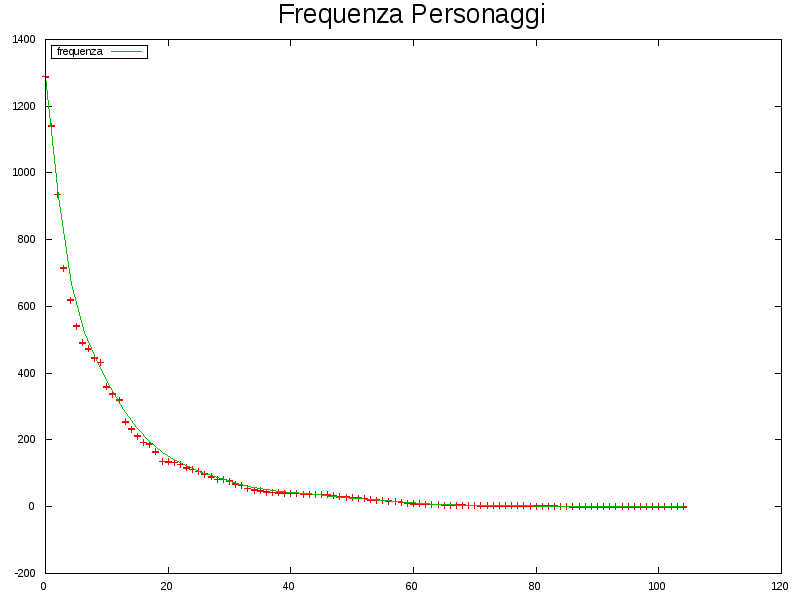
\includegraphics[width=.5\textwidth]{picture/frequenza_personaggi.png}
\caption{Grafico frequenza di ciascun personaggio nel romanzo}
\label{fig:frequenza-personaggi}
\end{figure}

La suddetta distribuzione segue una legge di potenza, ciò suggerisce una cricca di pochi personaggi determinanti e una rete più ampia di personaggi meno importanti. Questa configurazione segue il principio di Pareto, ovvero il 20\% dei personaggi appare più dell'80\% delle volte nel romanzo.\\
Per poter individuare univocamente questo sottoinsieme si è calcolato come segue 
\begin{align}
\sum\limits_{i=1}^n f(personaggio_i ) = 11743\\
x:11743=80:100\nonumber\\
x=11743*80/100\nonumber\\
x=9394,4\nonumber  
\end{align}

Risolta l'equazione x rappresenta l'80\% dei legami della rete, questi legami sono distribuiti su di un numero esiguo di personaggi per poterli individuare si sono trovati tutti quei personaggi per cui sommandoli insieme la loro somma desse 9394,4.
Tali personaggi appaiono nel romanzo con una frequenza superiore a 165, si è deciso di estendere a 135 includendo nell'insieme Lysa Tully poichè personaggio importante per la vicenda, ciò è corretto essendo la suddivisione 80/20 una scelta empirica è necessario contestualizzarla quanto più possibile per rappresentare il caso reale.\\

Fatto ciò si è poi individuato l'insieme delle triplette:\\
nodo evento [valore]\\
definita come\\
personaggio capitolo citazione\\
l'enlenco è stato importato in UciNet come NodeAttr l'insieme appare corretto e del tutto credibile.\\


Sfruttando le funzionalità di UciNet si è affiliato da una bimodale ad una monomodale sulle righe personaggi, scegliendo come modalita la somma dei prodotti incrociati, (Sums of cross-products), ovvero la somma dei prodotti binari degli attori rispetto agli eventi. Che è l'equivalente di dire i casi in cui vi è co-orrorrenza.\\

Degli attori imporati si è scelto di filtrare gli attori con meno di 135 occorrenze totali ovvero di conservare solo il 20\% dei personaggi i quali meglio rappresentano i personaggi chiave del romanzo, a questa principale scrematura si 

A questo grafo si è applicato un filtro rimuovendo tutti i legami di intensità inferiore a 680, grazie a questo espediente abbiamo rimosso dalla rete tutti quei collegamenti troppo esili per significare davvero un legame tra due personaggi. 
\begin{figure}[h]
\centering
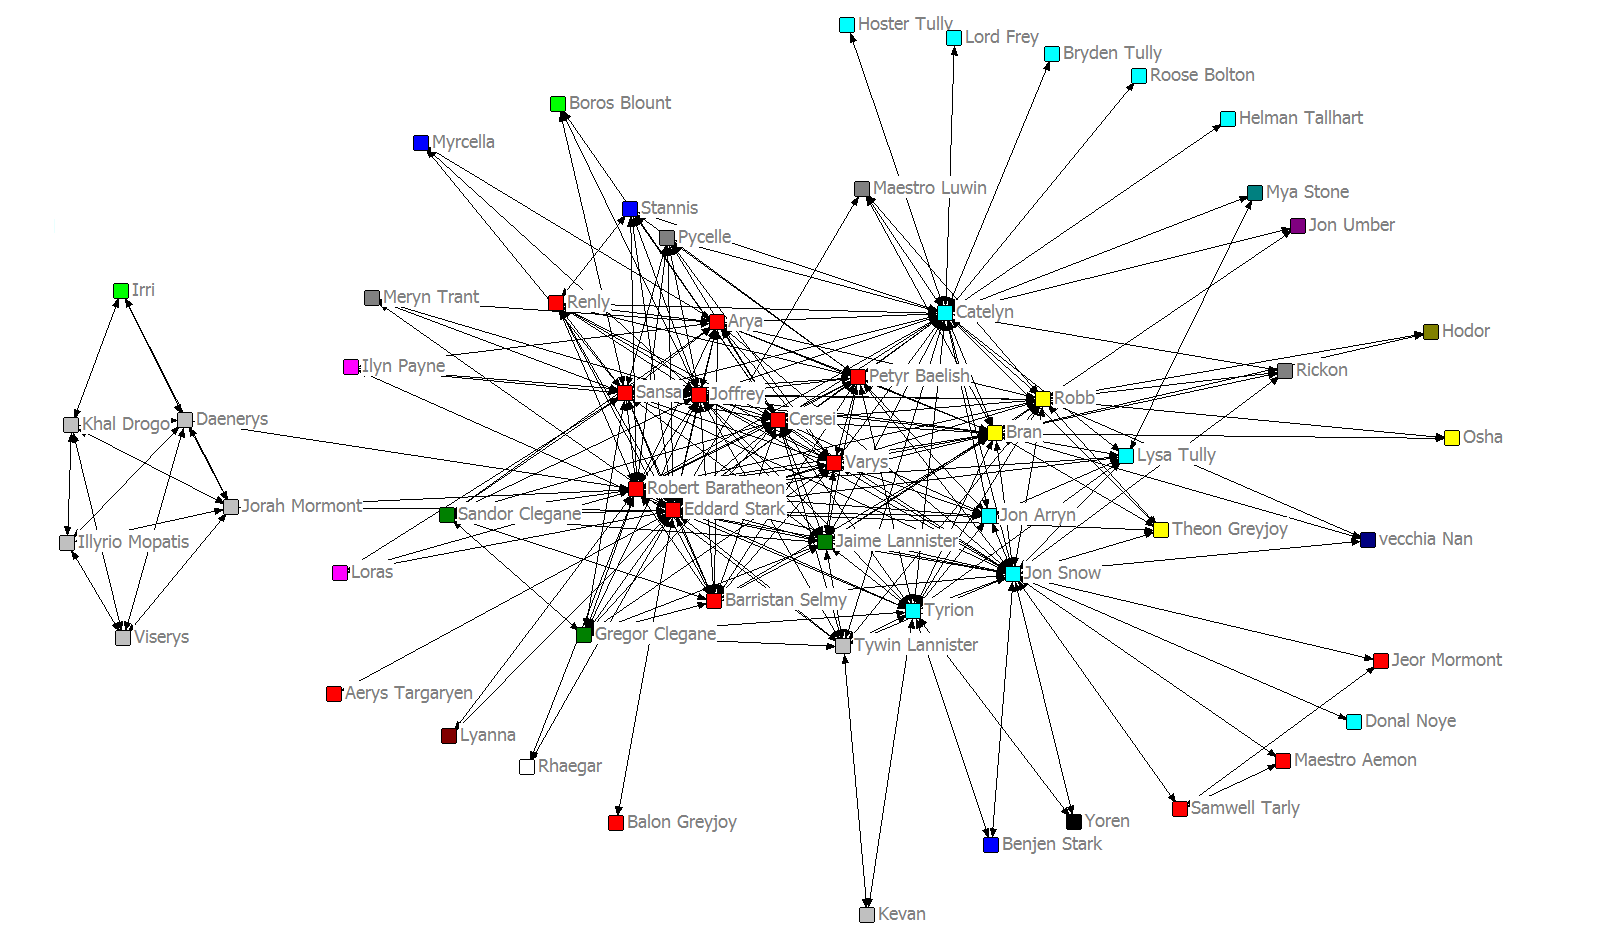
\includegraphics[width=.9\textwidth]{picture/029.png}
\caption{Il Grafo delle reti sociali}
\label{fig:grafo-partito}
\end{figure}
La rete presente in figura uno è stata colorata applicando il metodo di partizione della rete per fazioni, richiedendo al programma di cercare 20 fazioni all'interno della rete così filtrata.\\

\subsection{Casate}
Grazie al filtro per sottogruppi si è riuscito ad individuare quelle che a prima vista può apparire come le casate, ovvero le fazioni, presenti nel Trono di Spade.\\
Si è quindi scelto di analizzare numericamente quanto questa suddivisione riesca a catturare le reali casate del trono di spade.
\begin{itemize}
  \item \emph{Stark:} Eddard, Sansa, Arya, Bran, Robb, Rickon, Lyanna.
  \item \emph{Baratheon:} Robert, Renly, Stannis, Joffrey, Myrcella, Tommen.
  \item \emph{Lannister:} Tywin, Kevan, Cersei, Tyrion, Jaime.
  \item \emph{Tully:} Catelyn, Lysa, Hoster, Bryden.
  \item \emph{Targaryen:} Denerys, Viserys, Aerys, Rhaegar.
  \item \emph{Clegane:} Gregor, Sandor.
  \item \emph{Guardiani della Notte:} Jon Snow, Samwell Tarly, Meastro Aemon, Donal Noye, Jeor Mormont.
\end{itemize}

Fatta questa premessa possiamo verificare la corretta disposizione di 18 personaggi, la collocazione sbagliata di 18 personaggi e la mancata colorazione di 19 personaggi. (Figura \ref{fig:grafo-partito}) Essendo che alcuni personaggi colorati in modo errato risultano mancanti occorre rimuoverli dall'insieme dei personaggi sbagliati. Peranto risulta che vi sono 11 personaggi colorati in modo errato e 19 personaggi che dovevano essere colorati di un colore e che lo sono stati di un altro.\\ 
Da cui possiamo calcolare:

\begin{equation}
	p=1-\frac{19+11}{56}=0.46    
\end{equation}

Possiamo quindi concludere che la probabilità di individuare un personaggio corretto grazie a questa partizione del grafo è del 46\%, il che è un risultato piuttosto soddisfacente considerando che dividendo il gruppo casualmente in 7 fazioni la probabilità di colorare un elemento correttamente è del 14\%.\\

Alla luce di questa partizione bisogna valutare le incongruenze che emergono, sono giustificate?

Vi è una forte confusione tra gli Stark e i Lannister e i Baratheon, questo per via del fatto che questi personaggi si trasferiscono tutti ad Approdo del Re nel corso del romanzo e vivono una fitta trama ricca di alleanze e inimicizie sotterfugi e tradimenti.

Emerge che Jon Arryn è legato a Lysa Tully e ciò è ragionevole visto il loro legame matrimoniale, si può dire la medesima cosa di Kahal Drogo marito di Daenerys Targaryen.

Stannis e Renly Baratheon invece risultano ben divisi e ciò sarà ulteriormente evidente nei prossimi romanzi dove Stannis finrà per uccidere suo fratello Renly.

I guardiani della notte risultano un insieme non omogeneo giò è dovuto in parte anche al fatto che Benjen Stark sarà dato per disperso nelle prime pagine del libro e che Donal Noye ha un forte legame con Jon Snow.

Ultimo ma non meno importanza il legame tra Tyrion e il resto dei suoi parenti Tywin e Kevan è di evidente distacco, sappiamo che ha un legame con Catelyn Tully poichè ella lo prende come prigioniero e lo porta a Nido dell'Aquila da Lysa Tully.

\subsection{Relazioni Matrimoniali}

Si sono prese in considerazione le seguenti coppie:

\begin{itemize}
\item Khal Drogo - Daenerys Targaryen
\item Robert Baratheon - Cersei Lannister
\item Eddard Stark - Catelyn Tully
\item Jon Arryn - Lysa Tully
\end{itemize}

Ciascuno di questi legami matrimoniali è presente nella rete dicotomizzata a 680.\\
Per poter cogliere eventuali difficotà matrimoniali abbiamo dicotomizzato la rete a 1500 e ci siamo accorti che il legame tra Jon Arryn e Lysa Tully si spezza come in Figura \ref{fig:grafo-partito-1500}.\\
\begin{figure}[h]
\centering
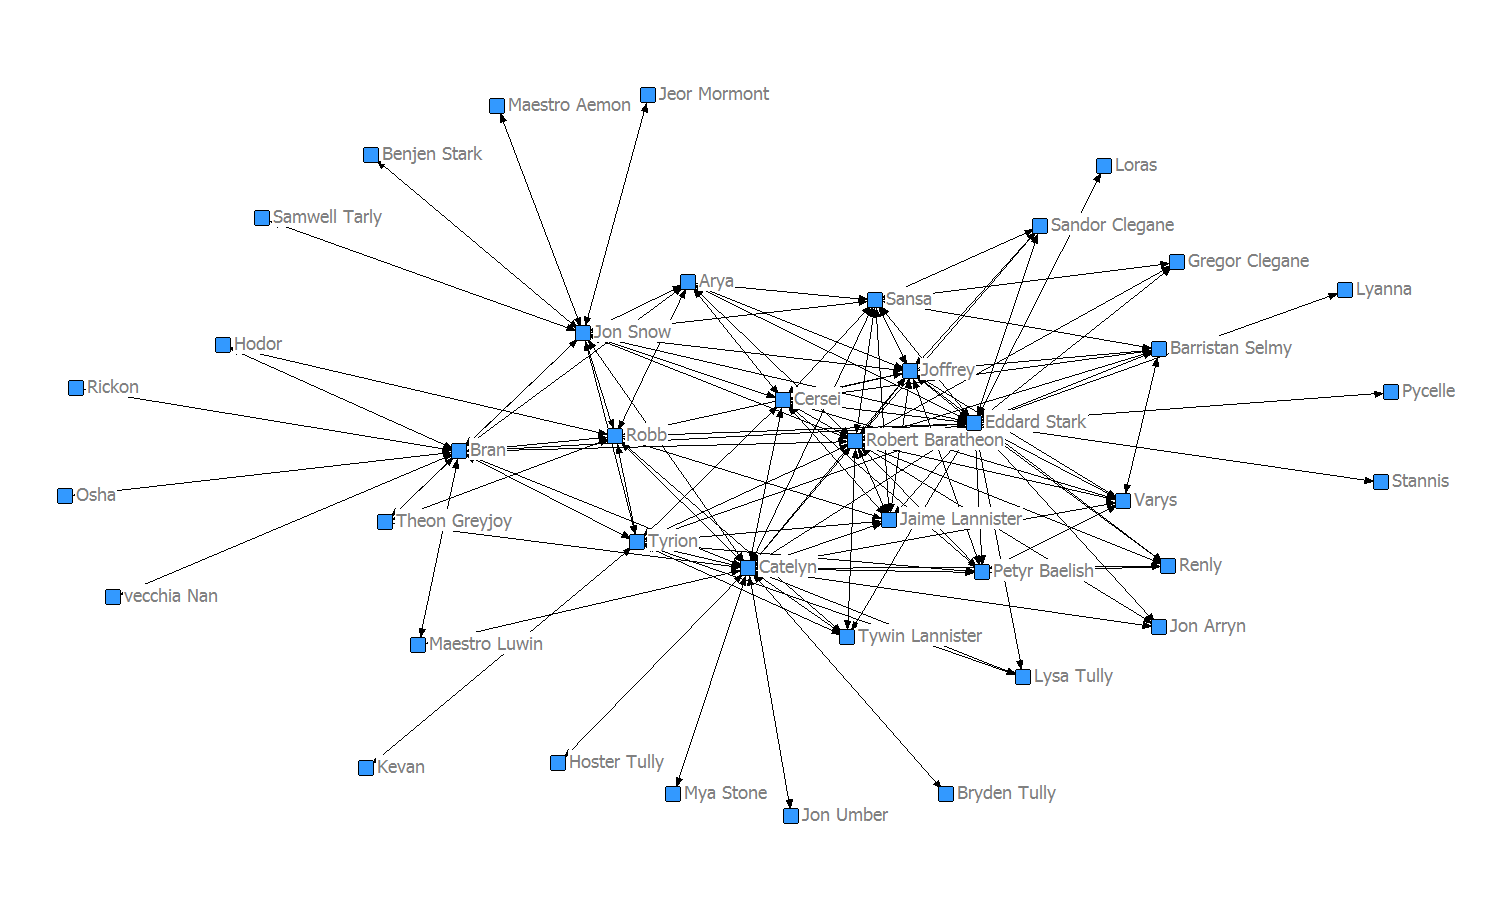
\includegraphics[width=.9\textwidth]{picture/030.png}
\caption{La componente principale del grafo dicotomizzato a 1500}
\label{fig:grafo-partito-1500}
\end{figure}
Per poter rompere altri legami matrimoniali bisogna spingersi a 5323 dove si spezza il legame tra Robert Baratheon e Cersei Lannister. Questo a prima vista può nascondere un errore di approccio, infatti sono così pochi i legami tra personaggi non "protagonisti" che lo spezzarsi di questo legame può apparire come una dipendnete di questo aspetto, quello che però non sarebbe spiegato è per quale motivo il rapporto tra Cersei e Joffrey suo figlio rimanga mentre quello tra marito e moglie si spezzi. Soltanto nella lettura del romanzo possiamo trovare risposta a questa evidenza empirica.






\section{Conclusioni}


\begin{thebibliography}{9}
  \bibitem{UciNet}
  	Borgatti, S.P., Everett, M.G. and Freeman, L.C. 2002. 		\emph{Ucinet for Windows: Software for Social Network Analysis. Harvard, MA: Analytic Technologies.} 
\end{thebibliography}

\end{document}